\section{Activités}

Le développement du projet peut se découper en plusieurs phases, qui elles-mêmes se divisent en plusieurs activités. Voici la liste de ces activités :

\begin{enumerate}
	\item Analyse des besoins
	\begin{enumerate}
		\item Analyse des features demandées
		\item Etude des cas d’utilisation
		\item Etude de la faisabilité des demandes
		\item Analyse de la correspondance avec la base de données existante
	\end{enumerate}
	\item Analyse des technologies
	\begin{enumerate}
		\item Analyse et choix des technologies pertinentes
		\item Apprentissage des technologies choisies
	\end{enumerate}
	\item Conception de l’application
	\begin{enumerate}
		\item Design de l’architecture générale de l’application
		\item Design de l’interaction et de la structure de navigation
		\item Prototypage
	\end{enumerate}
	\item Réalisation de l’application
	\begin{enumerate}
		\item Réalisation du code backend
		\item Réalisation du code frontend
		\item Evaluation du comportement fonctionnel de l’application
		\item Evaluation de la robustesse de l’application
	\end{enumerate}
	\item Evaluation itérative
	\begin{enumerate}
		\item Evaluation formative
		\item Evaluation sommative informelle et empirique
		\item Rétrospective du développement
	\end{enumerate}
\end{enumerate}

\section{Planification}
Le projet comporte une série de dates-clé qu’il est important de respecter :
\begin{center}
   \begin{tabular}{ | l | c | r | }
     \hline
		Date & Semaine & Tâche \\ \hline
		\color{red}Lundi 20 février 2017 & Semaine P1 & Début du projet \\ \hline
		Lundi 31 mars 2017 & Semaine P6 & Fin de l’apprentissage des technologies choisies \\ \hline
		Lundi 20 mai 2017 & Semaine P12 & Fin de l’implémentation de l’application \\ \hline
		\color{red}Vendredi 9 juin 2017 & Semaine P15 & Dépôt du rapport \\ \hline
		\color{red}19-30 juin 2017 & - & Défense orale \\ \hline
     \hline
   \end{tabular}
\end{center}

Les dates en rouge sont des dates de rendu officielles.
Les autres représentent des jalons dans l’avancement du projet.

\section{Diagramme de Gantt}
	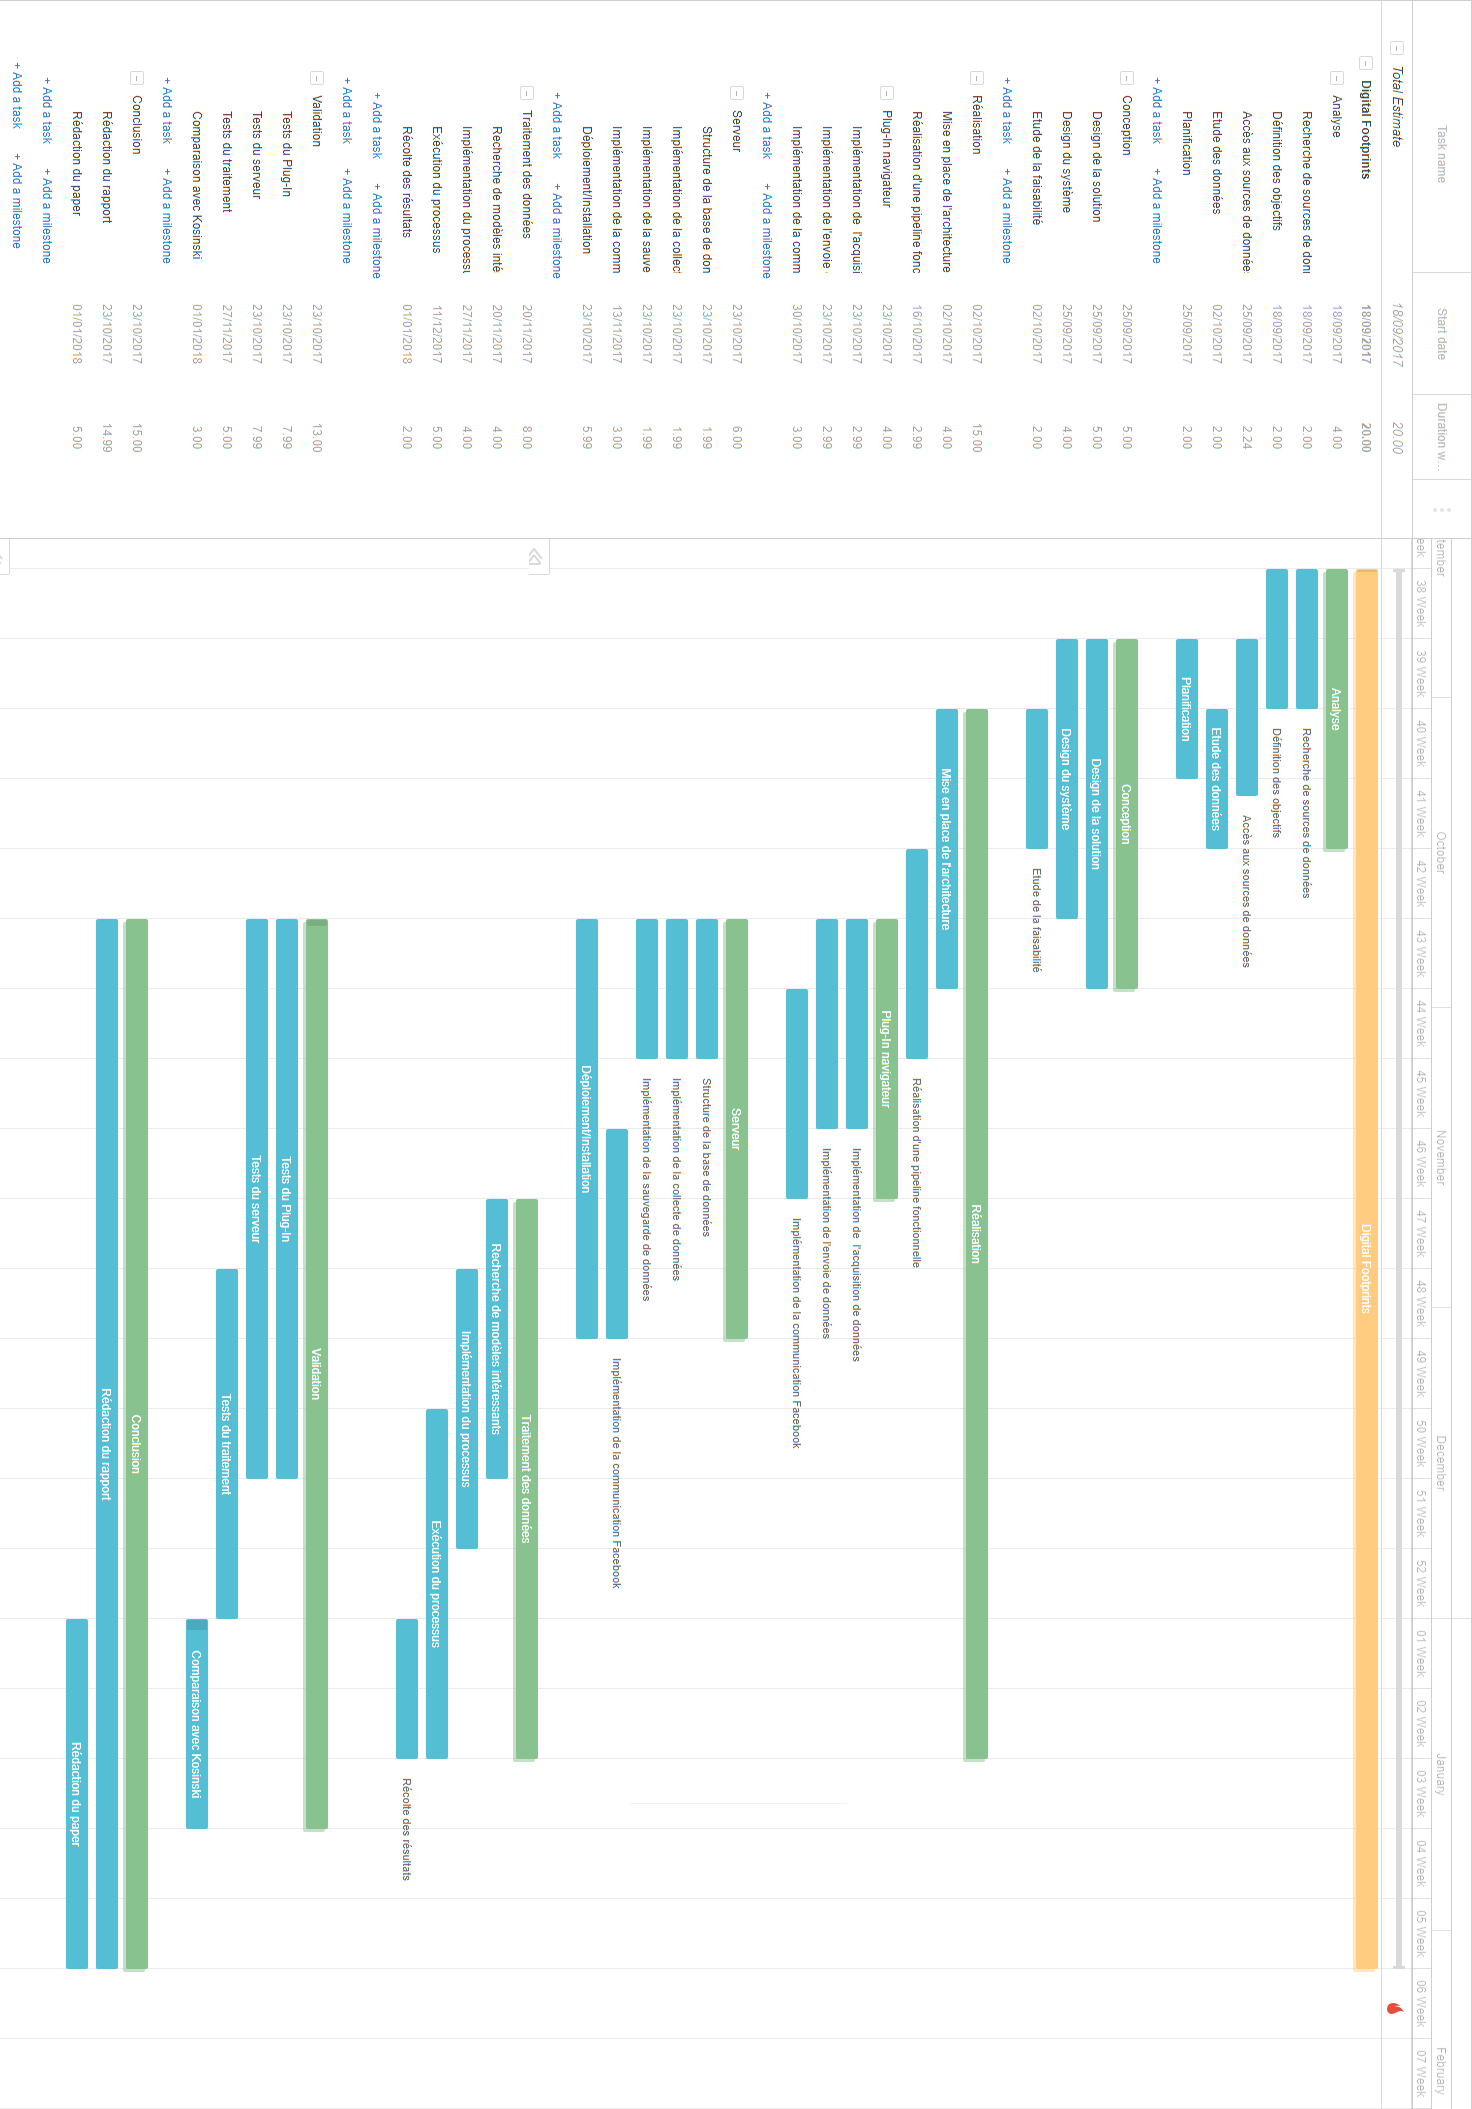
\includegraphics[width=0.51\textwidth]{images/annexes/cdc/gantt}